
%%%% Paramétrage du TD %%%%
\def\xxactivite{Application}
\def\xxauteur{\textsl{Xavier Pessoles}}


\def\xxnumchapitre{Chapitre 1 \vspace{.2cm}}
\def\xxchapitre{\hspace{.12cm} Stabilité des systèmes}

\def\xxcompetences{%
\textsl{%
\textbf{Savoirs et compétences :}\\
\vspace{-.4cm}
\begin{itemize}[label=\ding{112},font=\color{bleuxp}] 
%\item \textit{Mod3.C2 : } pôles dominants et réduction de l’ordre du modèle : principe, justification
%\item \textit{Res2.C4 : } stabilité des SLCI : définition entrée bornée -- sortie bornée (EB -- SB)	
%\item \textit{Res2.C5 : } stabilité des SLCI : équation caractéristique	
\item \textit{Res2.C6 : } stabilité des SLCI : position des pôles dans le plan complexe
\item \textit{Res2.C7 : } stabilité des SLCI : marges de stabilité (de gain et de phase)
\end{itemize}
}}


\def\xxfigures{
%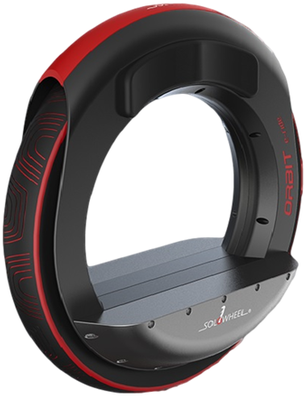
\includegraphics[width=3cm]{SoloWheel_Orbit}\\
%\textit{}
}%figues de la page de garde

\def\xxtitreexo{Application}
\def\xxsourceexo{\hspace{.2cm} \footnotesize{Xavier Pessoles}}


\def\xxactivite{Application \ifprof  -- Corrigé \else \fi}
%\def\xxauteur{\textsl{P. Dupas.}}


\iflivret
\input{\repRel/Style/pagegarde_TD}
\else
\input{\repRel/Style/pagegarde_TD}
\fi
\setlength{\columnseprule}{.1pt}

\pagestyle{fancy}
\thispagestyle{plain}


\vspace{4.5cm}

\def\columnseprulecolor{\color{bleuxp}}
\setlength{\columnseprule}{0.4pt} 

%%%%%%%%%%%%%%%%%%%%%%%


\setcounter{numques}{0}

\ifprof
\else
\begin{multicols}{2}
\question{On donne ci-dessous les lieux de transferts de plusieurs  FTBO. Déterminer, à l’aide du critère du Revers si les systèmes sont stables en BF. Pour les systèmes stables déterminer les marges de gain et de phase.}
\fi
 
\ifprof

\begin{center}
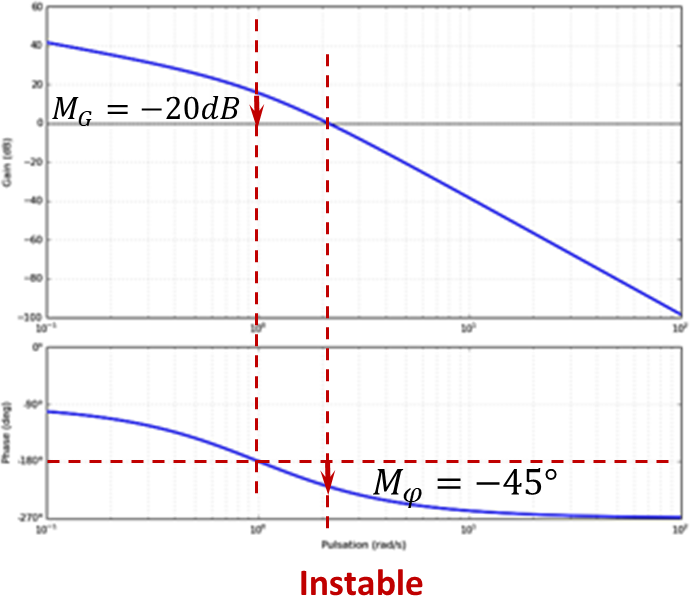
\includegraphics[width=8cm]{im_01_cor}
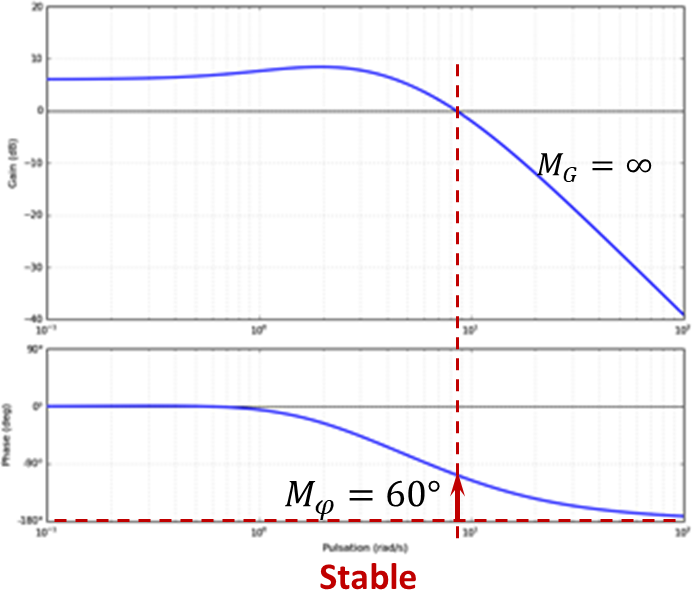
\includegraphics[width=8cm]{im_02_cor}
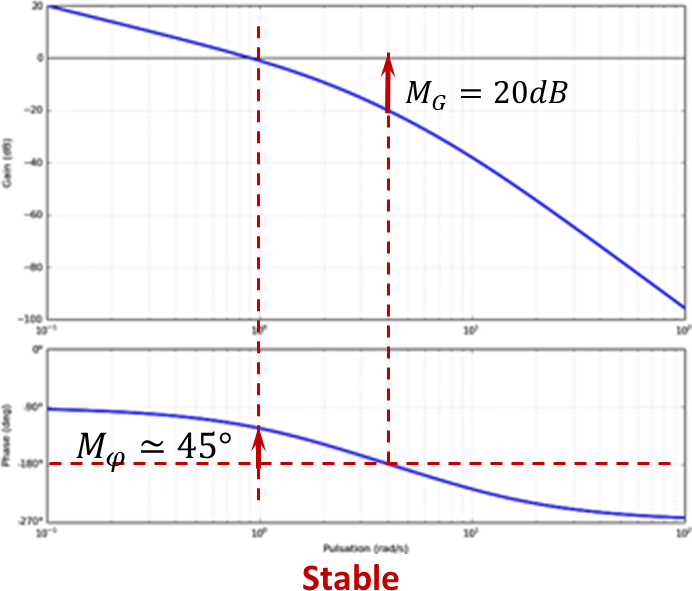
\includegraphics[width=8cm]{im_03_cor}
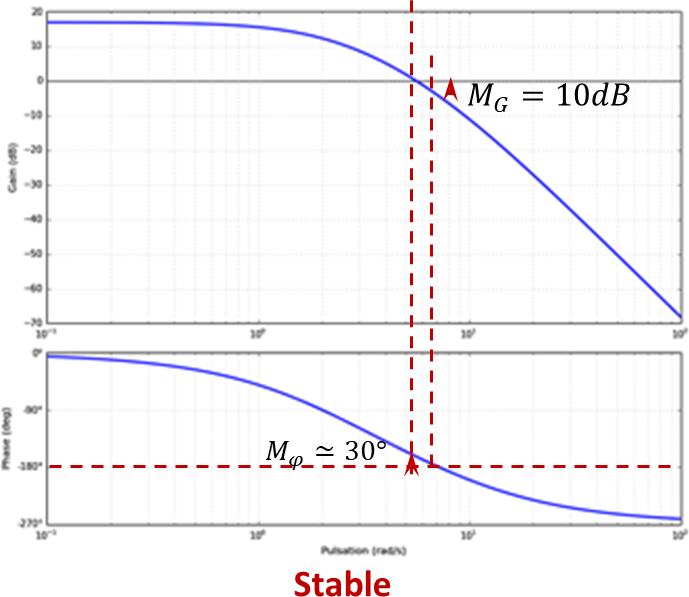
\includegraphics[width=8cm]{im_04_cor}
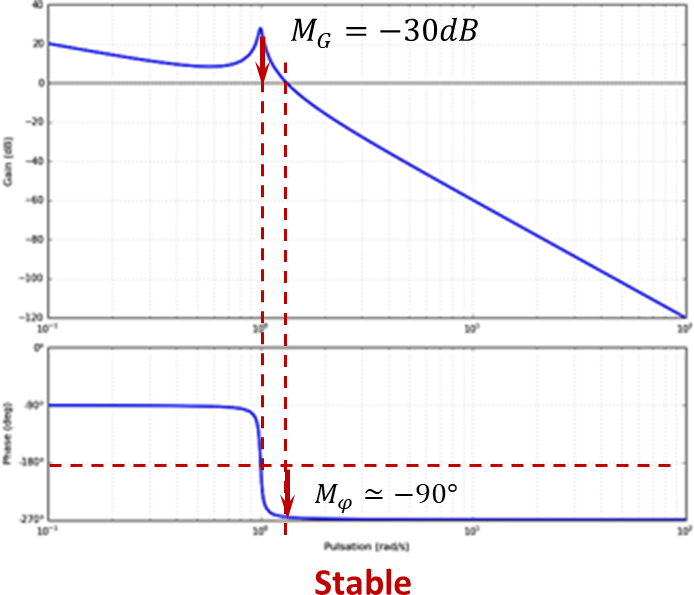
\includegraphics[width=8cm]{im_05_cor}
\end{center}

 \else
\begin{center}
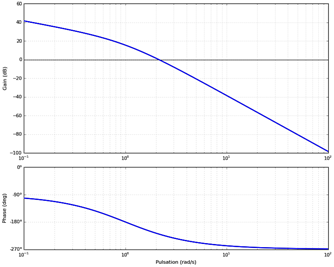
\includegraphics[width=\linewidth]{im_01}
\end{center}

\begin{center}
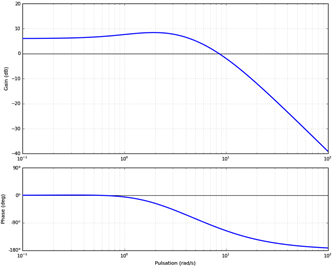
\includegraphics[width=\linewidth]{im_02}
\end{center}

\begin{center}
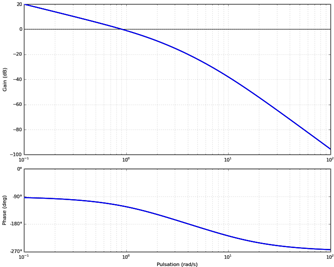
\includegraphics[width=.9\linewidth]{im_03}
\end{center}

\begin{center}
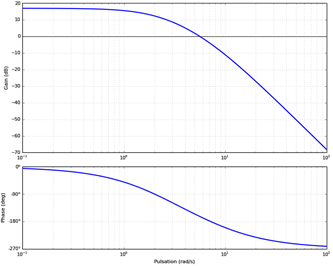
\includegraphics[width=.9\linewidth]{im_04}
\end{center}

\begin{center}
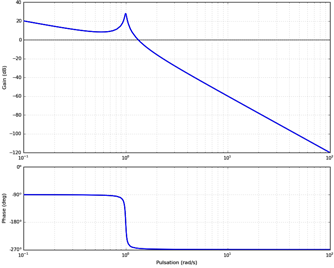
\includegraphics[width=.9\linewidth]{im_05}
\end{center}
\fi

\ifprof
\else
\end{multicols}
\fi


